%%%%%%%%%%%%%%%%%%%%%%%%%%%%%%%%%%%%%%%%%%%%%%%%%%%%%%%%%%%%%%%%%%%
%                                                                 %
%                            CHAPTER THREE                        %
%                                                                 %
%%%%%%%%%%%%%%%%%%%%%%%%%%%%%%%%%%%%%%%%%%%%%%%%%%%%%%%%%%%%%%%%%%%

\chapter{METHODOLOGY}\label{ch:model}

The goal of data set versioning is to expose the relationships between versions of a data set.
To do this, the concept model relates three kinds of --- objects, versions, attributes, and changes --- using three different orientations.
The model obviously includes versions because they are the objects being compared.
Identifying one object, however, as a version of another does not give much insight into the nature of their relationship.
In order to characterize the change between two versions, the model relates their attributes.
The model uses the Dublin Core Term \textit{dco:hasPart} to facilitate the link from a version to its attribute.
The changes used then defines the difference between these attributes in each version.
The modeling process can be viewed as creating a mapping between an original set and a new data set.
As mentioned previously, the operations conducted by data versioning systems boil down to primarily three operations: addition, invalidation, and modification.
Since these activities are so prevalent, we use these three procedures to characterize the relationships between versions.
A modification is straight forward to model because it maps together an attribute which exists in both versions, but addition and invalidation are a little different.
Because the attribute doesn't exist in one version or in the other for addition and invalidation, it forms a '0 to 1' relationship between the attributes.
This causes a problem technically because without a concept on one end, a mapping cannot be formed.
The chosen solution was to use the version concept as the anchor in place of the non-existent attribute.
This observation leads to the conceptual model's structure used in this dissertation.
The nature of change can be determined by observing the construction used to model a relationship and counting the number of attributes on each side.
As a note, the figures in this chapter only depict the attribute relationships as 0 to 1, 1 to 0, and 1 to 1 --- the cardinality of links entering a change concept from an attribute to the number of links exiting to an attribute.
It is more valid to consider the relationships as 0 to X, X to 0, and X to Y in cardinality because it may take more than one attribute to identify an observation in a version.
For example, a cell in tabular data would need a row and a column to identify it, or a modification may change a single location attribute into two separate latitude and longitude entries.

An obvious concern about using these requirements to determine the mapping is that it does not guarantee meaningful versioning is being performed.
In order to ensure that the relationships being exposed by the mapping are valid, we must go back to the definition of versions.
Having common provenance establishes that performing a comparison between these two objects results in a relation pertaining to the same application.
In addition, if the objects also can share the same workflow step it establishes that they have relatable content.
This also addresses the possibility that we are comparing objects that have different purposes at separate points in a workflow, but share provenance as a result.
Before applying the methods in this model, it must, therefore, be first established that the two objects satisfy the requirements to be versions of each other.

\section{Left-hand Right-hand Convention}

\section{Modification}

The simplest operation to model is \textit{modification} because it has no missing parts.
It maps a change from one attribute of version one to its corresponding attribute in version two.
In Figure \ref{ModificationFig}, a versioning comparison is being performed between two objects, Version 1 and Version 2.
Each version has an attribute, Attribute 1 and Attribute 2, respectively.
Finally, a change object connects the two attributes, denoting that the values described by the attribute are different.

\begin{figure}
	\centering
	\vspace{0.0in} % normally the command here would be \includegraphics
	%	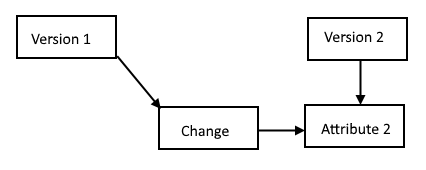
\includegraphics{figures/Addition.png}
	\begin{tikzpicture}[every node/.style={draw, rectangle}]
	\begin{scope}[node distance=20mm and 20mm]
	\node (c) [scale=1.25] at (1,0) {Change M};
	\node (1) [above left=of c, scale=1.25] {Version 1};
	\node (2) [above right=of c, scale=1.25] {Version 2};
	\node (a1) [below =of 1, scale=1.25] {Attribute 1};
	\node (a2) [below =of 2, scale=1.25] {Attribute 2};
	
	\draw [line width=2pt,->] (a1) -- (c);
	\draw [line width=2pt,->] (c) -- (a2);
	\draw [line width=2pt, ->] (1) -- (a1);
	\draw [line width=2pt, ->] (2) -- (a2);
	\end{scope}
	\end{tikzpicture}
	\caption{Model of the relationships between Versions 1 and 2 when modifying Attribute 1 from Version 1 as a result of Change M, resulting in Attribute 2 from Version 2}
	\label{ModificationFig}  % the \label command comes AFTER the caption
\end{figure}

Notice that the model captures neither the change's magnitude, nor the values of the attributes involved in the change.
These are not included because too much domain knowledge will be required to interpret the significance of the value.
In addition, the model would essentially begin storing a copy of the data set, leading to space and redundancy concerns.
If an application needs to include this information, they can be added as a property of the attributes involved, but this is outside the scope of this thesis.
Simply knowing that the attribute has changed provides valuable information to identify the relationship between the two attributes from a versioning standpoint.
Sometimes it may be necessary to distinguish between modification changes.
For this reason, the \textit{vo:Change} concept in this relationship may be sub-classed to differentiate between different kinds of change that map one attribute to another.
For example, in order to distinguish a modification in which the units of a measurement changes, a \textit{UnitChange} concept, which sub-classes the \textit{Modify} change concept, can be used to connect the attributes from two different version.



\section{Addition}

In Figure \ref{AdditionFig}, the \textit{addition} model differs from the \textit{modification} construction by the absence of Attribute 1.
This should mean that there does not exist a relationship between Version 1 and the concept Change A as the inclusion of Attribute 2 into Version 2 does not in general use content from the previous object.
Change A in this model, however, is not an activity, but a comparison relationship between Version 1 and 2.
A path, therefore, must exist from Version 1 to Attribute 2.
This formulation has the added benefit of conveying the idea of change as a quantity of flow, coming out of Version 1 and moving through the graph.
In this context, the structure establishes the left-hand version object as a source of flow when attributes become added to the following object.
This construction also forms a symmetric orientation with Invalidation.

\begin{figure}
	\centering
	\vspace{0.0in} % normally the command here would be \includegraphics
	%	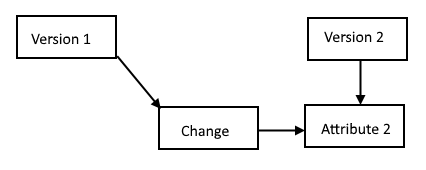
\includegraphics{figures/Addition.png}
	\begin{tikzpicture}[every node/.style={draw, rectangle}]
	\begin{scope}[node distance=20mm and 20mm]
	\node (c) [scale=1.25] at (1,0) {Change A};
	\node (1) [above left=of c, scale=1.25] {Version 1};
	\node (2) [above right=of c, scale=1.25] {Version 2};
	\node (a) [below =of 2, scale=1.25] {Attribute 2};
	
	\draw [line width=2pt,->] (1) -- (c);
	\draw [line width=2pt,->] (c) -- (a);
	\draw [line width=2pt, ->] (2) -- (a);
	\end{scope}
	\end{tikzpicture}
	\caption{Model of the relationships between Versions 1 and 2 when adding an Attribute 2 to Version 2 as a result of Change A}
	\label{AdditionFig}  % the \label command comes AFTER the caption
\end{figure}




\section{Invalidation}

The \textit{invalidation} relationship has a missing attribute object on the other side of the relation, contrary to the addition construction.
As a result of the invalidation, an attribute no longer exists in the following version.
As seen in Figure \ref{InvalidationFig}, the invalidation change concept matches to the Version 2 object.
Just like in addition model, this construction maintains a link between the two version objects.
In this case, it makes more conceptual sense, however, because Version 2 invalidates Attribute 1 by omitting it.

\begin{figure}
	\centering
	\vspace{0.0in} % normally the command here would be \includegraphics
	%	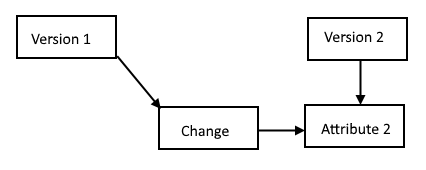
\includegraphics{figures/Addition.png}
	\begin{tikzpicture}[every node/.style={draw, rectangle}]
	\begin{scope}[node distance=15mm and 20mm]
	\node (c) [scale=1.25] at (1,0) {Change I};
	\node (1) [above left=of c, scale=1.25] {Version 1};
	\node (2) [above right=of c, scale=1.25] {Version 2};
	\node (a) [below =of 1, scale=1.25] {Attribute 1};
	
	\draw [line width=2pt,->] (a) -- (c);
	\draw [line width=2pt,->] (c) -- (2);
	\draw [line width=2pt, ->] (1) -- (a);
	\end{scope}
	\end{tikzpicture}
	\caption{Model of the relationships between Versions 1 and 2 when invalidating Attribute 1 from Version 1 as a result of Change I}
	\label{InvalidationFig}  % the \label command comes AFTER the caption
\end{figure}

